% !TEX TS-program = pdflatex
% !TEX encoding = UTF-8 Unicode
\documentclass[border=0mm]{standalone}
% packages
\usepackage{tikz}
\usetikzlibrary{patterns}
\usepackage{amsmath,amssymb}
\usepackage{bm}
\usepackage{pgfplots}
\pgfplotsset{compat=1.15}
% start document
\begin{document}
% generated by ROOT (CERN)
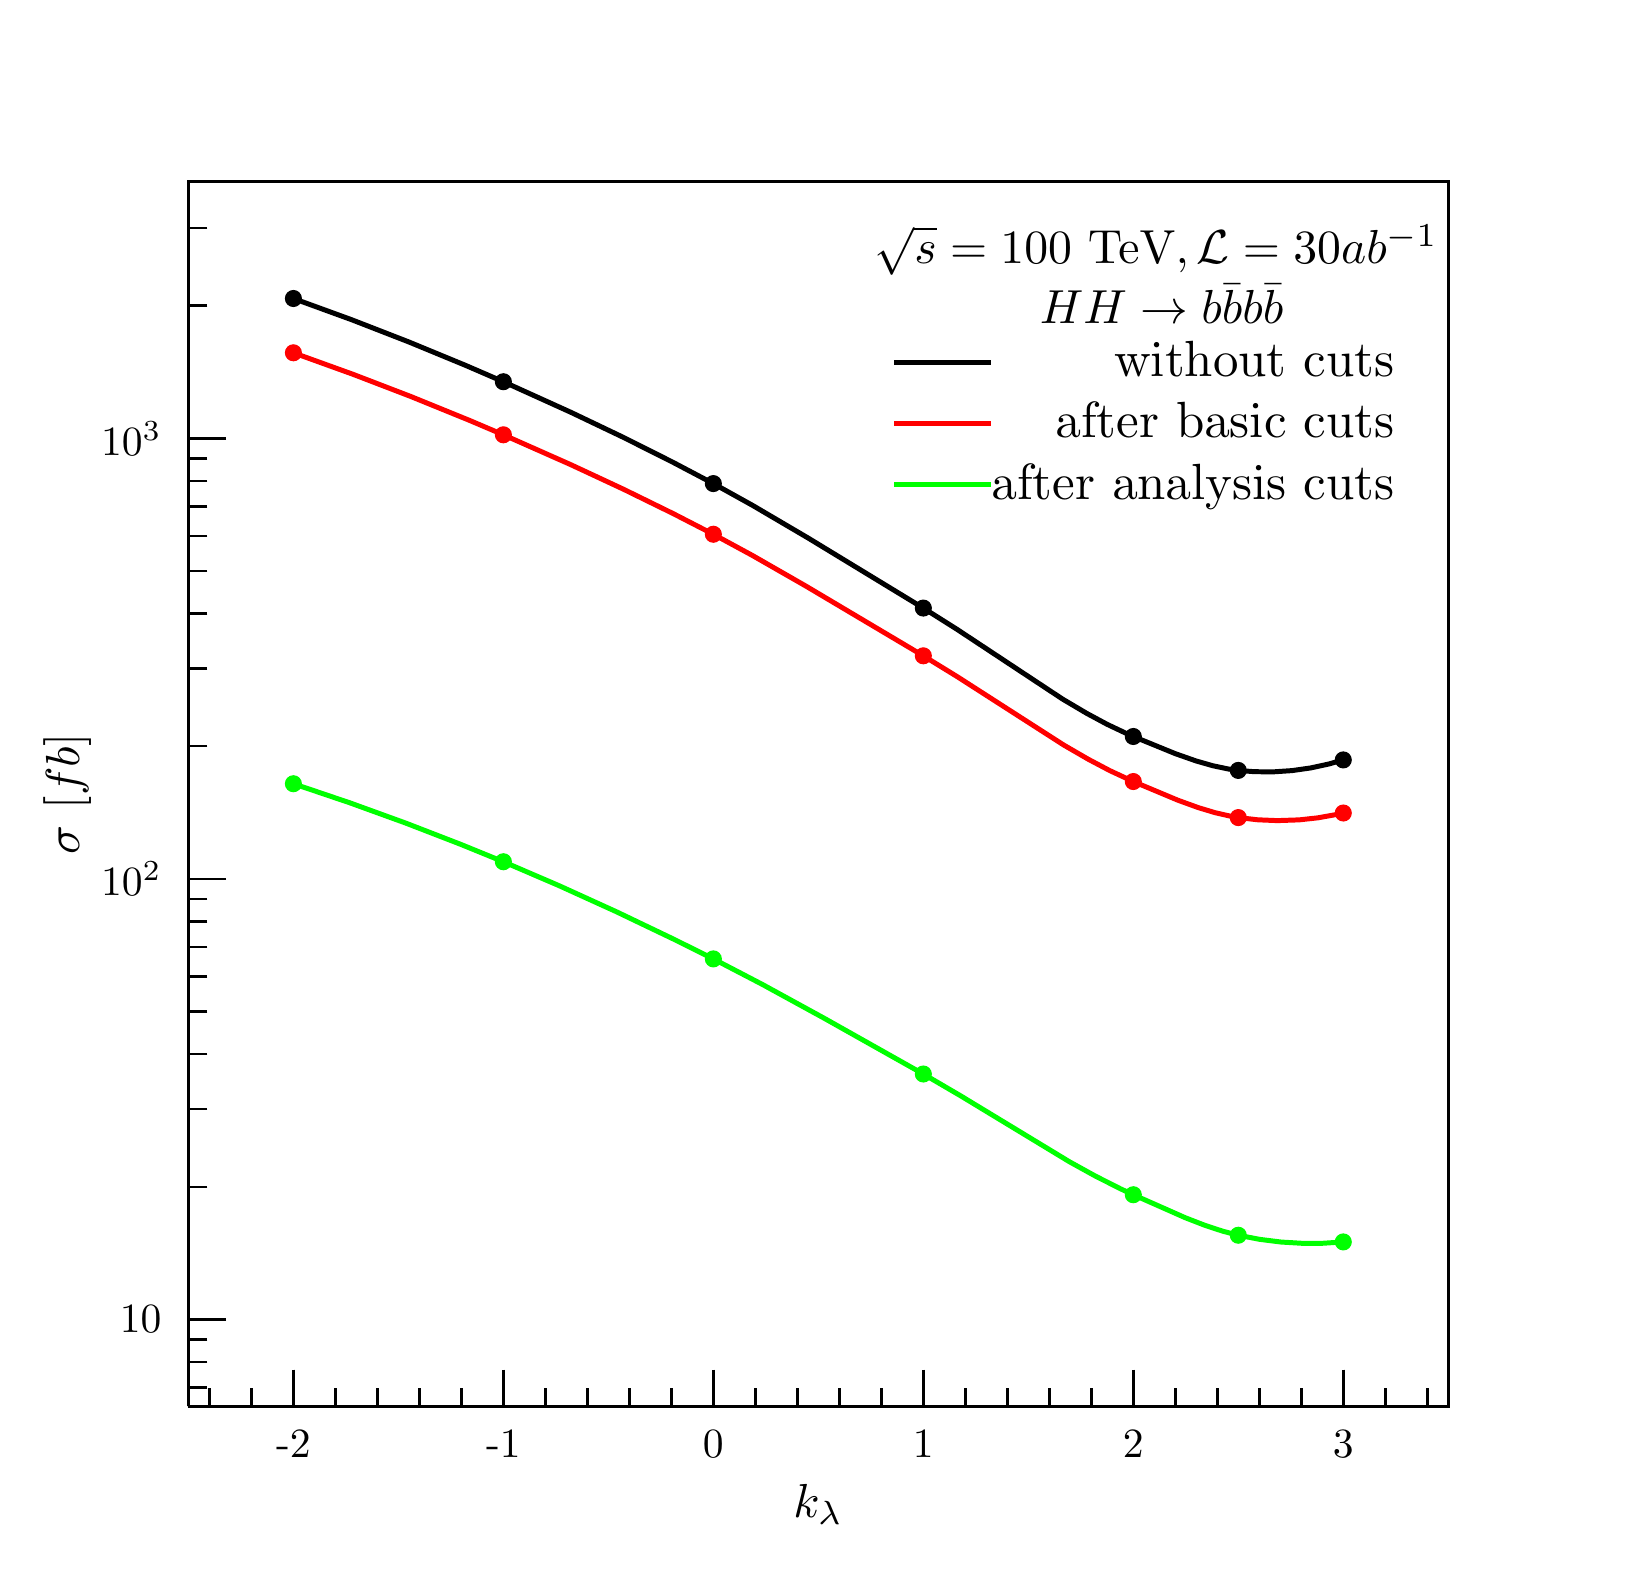
\begin{tikzpicture}
\pgfdeclareplotmark{cross} {
\pgfpathmoveto{\pgfpoint{-0.3\pgfplotmarksize}{\pgfplotmarksize}}
\pgfpathlineto{\pgfpoint{+0.3\pgfplotmarksize}{\pgfplotmarksize}}
\pgfpathlineto{\pgfpoint{+0.3\pgfplotmarksize}{0.3\pgfplotmarksize}}
\pgfpathlineto{\pgfpoint{+1\pgfplotmarksize}{0.3\pgfplotmarksize}}
\pgfpathlineto{\pgfpoint{+1\pgfplotmarksize}{-0.3\pgfplotmarksize}}
\pgfpathlineto{\pgfpoint{+0.3\pgfplotmarksize}{-0.3\pgfplotmarksize}}
\pgfpathlineto{\pgfpoint{+0.3\pgfplotmarksize}{-1.\pgfplotmarksize}}
\pgfpathlineto{\pgfpoint{-0.3\pgfplotmarksize}{-1.\pgfplotmarksize}}
\pgfpathlineto{\pgfpoint{-0.3\pgfplotmarksize}{-0.3\pgfplotmarksize}}
\pgfpathlineto{\pgfpoint{-1.\pgfplotmarksize}{-0.3\pgfplotmarksize}}
\pgfpathlineto{\pgfpoint{-1.\pgfplotmarksize}{0.3\pgfplotmarksize}}
\pgfpathlineto{\pgfpoint{-0.3\pgfplotmarksize}{0.3\pgfplotmarksize}}
\pgfpathclose
\pgfusepathqstroke
}
\pgfdeclareplotmark{cross*} {
\pgfpathmoveto{\pgfpoint{-0.3\pgfplotmarksize}{\pgfplotmarksize}}
\pgfpathlineto{\pgfpoint{+0.3\pgfplotmarksize}{\pgfplotmarksize}}
\pgfpathlineto{\pgfpoint{+0.3\pgfplotmarksize}{0.3\pgfplotmarksize}}
\pgfpathlineto{\pgfpoint{+1\pgfplotmarksize}{0.3\pgfplotmarksize}}
\pgfpathlineto{\pgfpoint{+1\pgfplotmarksize}{-0.3\pgfplotmarksize}}
\pgfpathlineto{\pgfpoint{+0.3\pgfplotmarksize}{-0.3\pgfplotmarksize}}
\pgfpathlineto{\pgfpoint{+0.3\pgfplotmarksize}{-1.\pgfplotmarksize}}
\pgfpathlineto{\pgfpoint{-0.3\pgfplotmarksize}{-1.\pgfplotmarksize}}
\pgfpathlineto{\pgfpoint{-0.3\pgfplotmarksize}{-0.3\pgfplotmarksize}}
\pgfpathlineto{\pgfpoint{-1.\pgfplotmarksize}{-0.3\pgfplotmarksize}}
\pgfpathlineto{\pgfpoint{-1.\pgfplotmarksize}{0.3\pgfplotmarksize}}
\pgfpathlineto{\pgfpoint{-0.3\pgfplotmarksize}{0.3\pgfplotmarksize}}
\pgfpathclose
\pgfusepathqfillstroke
}
\pgfdeclareplotmark{newstar} {
\pgfpathmoveto{\pgfqpoint{0pt}{\pgfplotmarksize}}
\pgfpathlineto{\pgfqpointpolar{44}{0.5\pgfplotmarksize}}
\pgfpathlineto{\pgfqpointpolar{18}{\pgfplotmarksize}}
\pgfpathlineto{\pgfqpointpolar{-20}{0.5\pgfplotmarksize}}
\pgfpathlineto{\pgfqpointpolar{-54}{\pgfplotmarksize}}
\pgfpathlineto{\pgfqpointpolar{-90}{0.5\pgfplotmarksize}}
\pgfpathlineto{\pgfqpointpolar{234}{\pgfplotmarksize}}
\pgfpathlineto{\pgfqpointpolar{198}{0.5\pgfplotmarksize}}
\pgfpathlineto{\pgfqpointpolar{162}{\pgfplotmarksize}}
\pgfpathlineto{\pgfqpointpolar{134}{0.5\pgfplotmarksize}}
\pgfpathclose
\pgfusepathqstroke
}
\pgfdeclareplotmark{newstar*} {
\pgfpathmoveto{\pgfqpoint{0pt}{\pgfplotmarksize}}
\pgfpathlineto{\pgfqpointpolar{44}{0.5\pgfplotmarksize}}
\pgfpathlineto{\pgfqpointpolar{18}{\pgfplotmarksize}}
\pgfpathlineto{\pgfqpointpolar{-20}{0.5\pgfplotmarksize}}
\pgfpathlineto{\pgfqpointpolar{-54}{\pgfplotmarksize}}
\pgfpathlineto{\pgfqpointpolar{-90}{0.5\pgfplotmarksize}}
\pgfpathlineto{\pgfqpointpolar{234}{\pgfplotmarksize}}
\pgfpathlineto{\pgfqpointpolar{198}{0.5\pgfplotmarksize}}
\pgfpathlineto{\pgfqpointpolar{162}{\pgfplotmarksize}}
\pgfpathlineto{\pgfqpointpolar{134}{0.5\pgfplotmarksize}}
\pgfpathclose
\pgfusepathqfillstroke
}
\definecolor{c}{rgb}{1,1,1};
\draw [color=c, fill=c] (0,0) rectangle (20,19.4486);
\draw [color=c, fill=c] (0,0) rectangle (20,19.4486);
\draw [color=c, fill=c] (2,1.94486) rectangle (18,17.5038);
\definecolor{c}{rgb}{0,0,0};
\draw [c,line width=0.9] (2,1.94486) -- (2,17.5038) -- (18,17.5038) -- (18,1.94486) -- (2,1.94486);
\definecolor{c}{rgb}{1,1,1};
\draw [color=c, fill=c] (2,1.94486) rectangle (18,17.5038);
\definecolor{c}{rgb}{0,0,0};
\draw [c,line width=0.9] (2,1.94486) -- (2,17.5038) -- (18,17.5038) -- (18,1.94486) -- (2,1.94486);
\definecolor{c}{rgb}{0,0,0.6};
\draw [c,line width=0.9] (2,1.94486) -- (2.16,1.94486) -- (2.16,1.94486) -- (2.32,1.94486) -- (2.32,1.94486) -- (2.48,1.94486) -- (2.48,1.94486) -- (2.64,1.94486) -- (2.64,1.94486) -- (2.8,1.94486) -- (2.8,1.94486) -- (2.96,1.94486) -- (2.96,1.94486)
 -- (3.12,1.94486) -- (3.12,1.94486) -- (3.28,1.94486) -- (3.28,1.94486) -- (3.44,1.94486) -- (3.44,1.94486) -- (3.6,1.94486) -- (3.6,1.94486) -- (3.76,1.94486) -- (3.76,1.94486) -- (3.92,1.94486) -- (3.92,1.94486) -- (4.08,1.94486) -- (4.08,1.94486)
 -- (4.24,1.94486) -- (4.24,1.94486) -- (4.4,1.94486) -- (4.4,1.94486) -- (4.56,1.94486) -- (4.56,1.94486) -- (4.72,1.94486) -- (4.72,1.94486) -- (4.88,1.94486) -- (4.88,1.94486) -- (5.04,1.94486) -- (5.04,1.94486) -- (5.2,1.94486) -- (5.2,1.94486)
 -- (5.36,1.94486) -- (5.36,1.94486) -- (5.52,1.94486) -- (5.52,1.94486) -- (5.68,1.94486) -- (5.68,1.94486) -- (5.84,1.94486) -- (5.84,1.94486) -- (6,1.94486) -- (6,1.94486) -- (6.16,1.94486) -- (6.16,1.94486) -- (6.32,1.94486) -- (6.32,1.94486) --
 (6.48,1.94486) -- (6.48,1.94486) -- (6.64,1.94486) -- (6.64,1.94486) -- (6.8,1.94486) -- (6.8,1.94486) -- (6.96,1.94486) -- (6.96,1.94486) -- (7.12,1.94486) -- (7.12,1.94486) -- (7.28,1.94486) -- (7.28,1.94486) -- (7.44,1.94486) -- (7.44,1.94486) --
 (7.6,1.94486) -- (7.6,1.94486) -- (7.76,1.94486) -- (7.76,1.94486) -- (7.92,1.94486) -- (7.92,1.94486) -- (8.08,1.94486) -- (8.08,1.94486) -- (8.24,1.94486) -- (8.24,1.94486) -- (8.4,1.94486) -- (8.4,1.94486) -- (8.56,1.94486) -- (8.56,1.94486) --
 (8.72,1.94486) -- (8.72,1.94486) -- (8.88,1.94486) -- (8.88,1.94486) -- (9.04,1.94486) -- (9.04,1.94486) -- (9.2,1.94486) -- (9.2,1.94486) -- (9.36,1.94486) -- (9.36,1.94486) -- (9.52,1.94486) -- (9.52,1.94486) -- (9.68,1.94486) -- (9.68,1.94486) --
 (9.84,1.94486) -- (9.84,1.94486) -- (10,1.94486) -- (10,1.94486) -- (10.16,1.94486) -- (10.16,1.94486) -- (10.32,1.94486) -- (10.32,1.94486) -- (10.48,1.94486) -- (10.48,1.94486) -- (10.64,1.94486) -- (10.64,1.94486) -- (10.8,1.94486) --
 (10.8,1.94486) -- (10.96,1.94486) -- (10.96,1.94486) -- (11.12,1.94486) -- (11.12,1.94486) -- (11.28,1.94486) -- (11.28,1.94486) -- (11.44,1.94486) -- (11.44,1.94486) -- (11.6,1.94486) -- (11.6,1.94486) -- (11.76,1.94486) -- (11.76,1.94486) --
 (11.92,1.94486) -- (11.92,1.94486) -- (12.08,1.94486) -- (12.08,1.94486) -- (12.24,1.94486) -- (12.24,1.94486) -- (12.4,1.94486) -- (12.4,1.94486) -- (12.56,1.94486) -- (12.56,1.94486) -- (12.72,1.94486) -- (12.72,1.94486) -- (12.88,1.94486) --
 (12.88,1.94486) -- (13.04,1.94486) -- (13.04,1.94486) -- (13.2,1.94486) -- (13.2,1.94486) -- (13.36,1.94486) -- (13.36,1.94486) -- (13.52,1.94486) -- (13.52,1.94486) -- (13.68,1.94486) -- (13.68,1.94486) -- (13.84,1.94486) -- (13.84,1.94486) --
 (14,1.94486) -- (14,1.94486) -- (14.16,1.94486) -- (14.16,1.94486) -- (14.32,1.94486) -- (14.32,1.94486) -- (14.48,1.94486) -- (14.48,1.94486) -- (14.64,1.94486) -- (14.64,1.94486) -- (14.8,1.94486) -- (14.8,1.94486) -- (14.96,1.94486) --
 (14.96,1.94486) -- (15.12,1.94486) -- (15.12,1.94486) -- (15.28,1.94486) -- (15.28,1.94486) -- (15.44,1.94486) -- (15.44,1.94486) -- (15.6,1.94486) -- (15.6,1.94486) -- (15.76,1.94486) -- (15.76,1.94486) -- (15.92,1.94486) -- (15.92,1.94486) --
 (16.08,1.94486) -- (16.08,1.94486) -- (16.24,1.94486) -- (16.24,1.94486) -- (16.4,1.94486) -- (16.4,1.94486) -- (16.56,1.94486) -- (16.56,1.94486) -- (16.72,1.94486) -- (16.72,1.94486) -- (16.88,1.94486) -- (16.88,1.94486) -- (17.04,1.94486) --
 (17.04,1.94486) -- (17.2,1.94486) -- (17.2,1.94486) -- (17.36,1.94486) -- (17.36,1.94486) -- (17.52,1.94486) -- (17.52,1.94486) -- (17.68,1.94486) -- (17.68,1.94486) -- (17.84,1.94486) -- (17.84,1.94486) -- (18,1.94486);
\definecolor{c}{rgb}{0,0,0};
\draw [c,line width=0.9] (2,1.94486) -- (18,1.94486);
\draw [c,line width=0.9] (3.33333,2.41163) -- (3.33333,1.94486);
\draw [c,line width=0.9] (3.86667,2.17825) -- (3.86667,1.94486);
\draw [c,line width=0.9] (4.4,2.17825) -- (4.4,1.94486);
\draw [c,line width=0.9] (4.93333,2.17825) -- (4.93333,1.94486);
\draw [c,line width=0.9] (5.46667,2.17825) -- (5.46667,1.94486);
\draw [c,line width=0.9] (6,2.41163) -- (6,1.94486);
\draw [c,line width=0.9] (6.53333,2.17825) -- (6.53333,1.94486);
\draw [c,line width=0.9] (7.06667,2.17825) -- (7.06667,1.94486);
\draw [c,line width=0.9] (7.6,2.17825) -- (7.6,1.94486);
\draw [c,line width=0.9] (8.13333,2.17825) -- (8.13333,1.94486);
\draw [c,line width=0.9] (8.66667,2.41163) -- (8.66667,1.94486);
\draw [c,line width=0.9] (9.2,2.17825) -- (9.2,1.94486);
\draw [c,line width=0.9] (9.73333,2.17825) -- (9.73333,1.94486);
\draw [c,line width=0.9] (10.2667,2.17825) -- (10.2667,1.94486);
\draw [c,line width=0.9] (10.8,2.17825) -- (10.8,1.94486);
\draw [c,line width=0.9] (11.3333,2.41163) -- (11.3333,1.94486);
\draw [c,line width=0.9] (11.8667,2.17825) -- (11.8667,1.94486);
\draw [c,line width=0.9] (12.4,2.17825) -- (12.4,1.94486);
\draw [c,line width=0.9] (12.9333,2.17825) -- (12.9333,1.94486);
\draw [c,line width=0.9] (13.4667,2.17825) -- (13.4667,1.94486);
\draw [c,line width=0.9] (14,2.41163) -- (14,1.94486);
\draw [c,line width=0.9] (14.5333,2.17825) -- (14.5333,1.94486);
\draw [c,line width=0.9] (15.0667,2.17825) -- (15.0667,1.94486);
\draw [c,line width=0.9] (15.6,2.17825) -- (15.6,1.94486);
\draw [c,line width=0.9] (16.1333,2.17825) -- (16.1333,1.94486);
\draw [c,line width=0.9] (16.6667,2.41163) -- (16.6667,1.94486);
\draw [c,line width=0.9] (3.33333,2.41163) -- (3.33333,1.94486);
\draw [c,line width=0.9] (2.8,2.17825) -- (2.8,1.94486);
\draw [c,line width=0.9] (2.26667,2.17825) -- (2.26667,1.94486);
\draw [c,line width=0.9] (16.6667,2.41163) -- (16.6667,1.94486);
\draw [c,line width=0.9] (17.2,2.17825) -- (17.2,1.94486);
\draw [c,line width=0.9] (17.7333,2.17825) -- (17.7333,1.94486);
\draw [anchor=base] (3.33333,1.30306) node[scale=1.50291, color=c, rotate=0]{-2};
\draw [anchor=base] (6,1.30306) node[scale=1.50291, color=c, rotate=0]{-1};
\draw [anchor=base] (8.66667,1.30306) node[scale=1.50291, color=c, rotate=0]{0};
\draw [anchor=base] (11.3333,1.30306) node[scale=1.50291, color=c, rotate=0]{1};
\draw [anchor=base] (14,1.30306) node[scale=1.50291, color=c, rotate=0]{2};
\draw [anchor=base] (16.6667,1.30306) node[scale=1.50291, color=c, rotate=0]{3};
\draw (10,0.700151) node[scale=1.72557, color=c, rotate=0]{$k_{\lambda}$};
\draw [c,line width=0.9] (2,1.94486) -- (2,17.5038);
\draw [c,line width=0.9] (2.24,2.18369) -- (2,2.18369);
\draw [c,line width=0.9] (2.24,2.50816) -- (2,2.50816);
\draw [c,line width=0.9] (2.24,2.79436) -- (2,2.79436);
\draw [c,line width=0.9] (2.48,3.05038) -- (2,3.05038);
\draw [anchor= east] (1.844,3.05038) node[scale=1.50291, color=c, rotate=0]{10};
\draw [c,line width=0.9] (2.24,4.73467) -- (2,4.73467);
\draw [c,line width=0.9] (2.24,5.71991) -- (2,5.71991);
\draw [c,line width=0.9] (2.24,6.41896) -- (2,6.41896);
\draw [c,line width=0.9] (2.24,6.96118) -- (2,6.96118);
\draw [c,line width=0.9] (2.24,7.4042) -- (2,7.4042);
\draw [c,line width=0.9] (2.24,7.77878) -- (2,7.77878);
\draw [c,line width=0.9] (2.24,8.10325) -- (2,8.10325);
\draw [c,line width=0.9] (2.24,8.38945) -- (2,8.38945);
\draw [c,line width=0.9] (2.48,8.64547) -- (2,8.64547);
\draw [anchor= east] (1.844,8.64547) node[scale=1.50291, color=c, rotate=0]{$10^{2}$};
\draw [c,line width=0.9] (2.24,10.3298) -- (2,10.3298);
\draw [c,line width=0.9] (2.24,11.315) -- (2,11.315);
\draw [c,line width=0.9] (2.24,12.014) -- (2,12.014);
\draw [c,line width=0.9] (2.24,12.5563) -- (2,12.5563);
\draw [c,line width=0.9] (2.24,12.9993) -- (2,12.9993);
\draw [c,line width=0.9] (2.24,13.3739) -- (2,13.3739);
\draw [c,line width=0.9] (2.24,13.6983) -- (2,13.6983);
\draw [c,line width=0.9] (2.24,13.9845) -- (2,13.9845);
\draw [c,line width=0.9] (2.48,14.2406) -- (2,14.2406);
\draw [anchor= east] (1.844,14.2406) node[scale=1.50291, color=c, rotate=0]{$10^{3}$};
\draw [c,line width=0.9] (2.24,15.9249) -- (2,15.9249);
\draw [c,line width=0.9] (2.24,16.9101) -- (2,16.9101);
\draw (0.464,9.72431) node[scale=1.72557, color=c, rotate=90]{$\sigma ~[fb]$};
\draw [c,line width=1.8] (3.33333,16.0159) -- (4.07134,15.7471) -- (4.79441,15.4661) -- (5.51779,15.1676) -- (6,14.959) -- (6.85855,14.5701) -- (7.52294,14.2528) -- (8.15166,13.9369) -- (8.66667,13.6654) -- (9.16568,13.3881) -- (9.87393,12.972) --
 (11.3333,12.0844) -- (11.7621,11.8139) -- (13.1021,10.9284) -- (13.4093,10.7468) -- (13.6678,10.608) -- (13.9291,10.484) -- (14,10.4535) -- (14.534,10.2353) -- (14.7987,10.1423) -- (15.008,10.0825) -- (15.211,10.0397) -- (15.3333,10.0225) --
 (15.5392,10.0063) -- (15.7767,10.0042) -- (16.0157,10.0203) -- (16.2533,10.0542) -- (16.485,10.1045) -- (16.6667,10.1559);
\foreach \P in {(3.33333,16.0159), (6,14.959), (8.66667,13.6654), (11.3333,12.0844), (14,10.4535), (15.3333,10.0225), (16.6667,10.1559)}{\draw[mark options={color=c,fill=c},mark size=2.882883pt,mark=*] plot coordinates {\P};}
\definecolor{c}{rgb}{1,0,0};
\draw [c,line width=1.8] (3.33333,15.3265) -- (4.08929,15.0537) -- (4.82306,14.772) -- (5.57056,14.4677) -- (6,14.285) -- (6.86095,13.9035) -- (7.52694,13.5929) -- (8.15525,13.2849) -- (8.66667,13.0218) -- (9.1625,12.7529) -- (9.84269,12.3633) --
 (11.3333,11.4782) -- (11.7687,11.2104) -- (13.1161,10.3452) -- (13.4274,10.165) -- (13.6993,10.0214) -- (14,9.88141) -- (14.5651,9.64472) -- (14.8254,9.55018) -- (15.0378,9.48612) -- (15.2494,9.43781) -- (15.3333,9.42368) -- (15.5823,9.39539) --
 (15.8304,9.38509) -- (16.108,9.39471) -- (16.3436,9.4204) -- (16.592,9.46493) -- (16.6667,9.4818);
\foreach \P in {(3.33333,15.3265), (6,14.285), (8.66667,13.0218), (11.3333,11.4782), (14,9.88141), (15.3333,9.42368), (16.6667,9.4818)}{\draw[mark options={color=c,fill=c},mark size=2.882883pt,mark=*] plot coordinates {\P};}
\definecolor{c}{rgb}{0,1,0};
\draw [c,line width=1.8] (3.33333,9.85359) -- (4.05124,9.61078) -- (4.76393,9.35232) -- (5.46048,9.08293) -- (6,8.86287) -- (6.70659,8.5592) -- (7.43419,8.22842) -- (8.16762,7.87738) -- (8.66667,7.62891) -- (9.28903,7.30486) -- (10.0839,6.86999) --
 (11.3333,6.16703) -- (11.8072,5.89013) -- (13.1879,5.05351) -- (13.5158,4.87229) -- (13.835,4.71054) -- (14,4.63389) -- (14.6603,4.34184) -- (14.9103,4.24503) -- (15.1372,4.17046) -- (15.3333,4.11936) -- (15.6054,4.0672) -- (15.8757,4.03311) --
 (16.1532,4.01645) -- (16.4111,4.01764) -- (16.6667,4.03467);
\foreach \P in {(3.33333,9.85359), (6,8.86287), (8.66667,7.62891), (11.3333,6.16703), (14,4.63389), (15.3333,4.11936), (16.6667,4.03467)}{\draw[mark options={color=c,fill=c},mark size=2.882883pt,mark=*] plot coordinates {\P};}
\definecolor{c}{rgb}{0,0,0};
\draw [anchor=base east] (17.5445,15.0241) node[scale=1.83926, color=c, rotate=0]{without cuts};
\draw [c,line width=1.8] (10.9633,15.2088) -- (12.1917,15.2088);
\draw [anchor=base east] (17.5445,14.2461) node[scale=1.83926, color=c, rotate=0]{after basic cuts};
\definecolor{c}{rgb}{1,0,0};
\draw [c,line width=1.8] (10.9633,14.4309) -- (12.1917,14.4309);
\definecolor{c}{rgb}{0,0,0};
\draw [anchor=base east] (17.5445,13.4682) node[scale=1.83926, color=c, rotate=0]{after analysis cuts};
\definecolor{c}{rgb}{0,1,0};
\draw [c,line width=1.8] (10.9633,13.6529) -- (12.1917,13.6529);
\definecolor{c}{rgb}{0,0,0};
\draw [anchor= west] (10.5,16.6286) node[scale=1.72557, color=c, rotate=0]{$\sqrt{s} = 100 ~\text{TeV}, \mathcal{L} = 30 ab^{-1}$};
\draw [anchor= west] (12.6,15.9479) node[scale=1.72557, color=c, rotate=0]{$HH \rightarrow b\bar{b}b\bar{b}$};
\end{tikzpicture}
% end document
\end{document}
